\documentclass[review]{elsarticle}

\usepackage{amsmath}
\usepackage{booktabs}
\usepackage{subcaption}
\usepackage{tabularx}
\usepackage{nicefrac}
\usepackage[usenames]{xcolor}
\usepackage{lineno,hyperref}
\modulolinenumbers[5]

\journal{Engineering Fracture Mechanics}

%%%%%%%%%%%%%%%%%%%%%%%
%% Elsevier bibliography styles
%%%%%%%%%%%%%%%%%%%%%%%
%% To change the style, put a % in front of the second line of the current style and
%% remove the % from the second line of the style you would like to use.
%%%%%%%%%%%%%%%%%%%%%%%

%% Numbered
%\bibliographystyle{model1-num-names}

%% Numbered without titles
%\bibliographystyle{model1a-num-names}

%% Harvard
%\bibliographystyle{model2-names.bst}\biboptions{authoryear}

%% Vancouver numbered
%\usepackage{numcompress}\bibliographystyle{model3-num-names}

%% Vancouver name/year
%\usepackage{numcompress}\bibliographystyle{model4-names}\biboptions{authoryear}

%% APA style
%\bibliographystyle{model5-names}\biboptions{authoryear}

%% AMA style
%\usepackage{numcompress}\bibliographystyle{model6-num-names}

%% `Elsevier LaTeX' style
\bibliographystyle{elsarticle-num}
%%%%%%%%%%%%%%%%%%%%%%%

\begin{document}

\begin{frontmatter}

\title{Finite Element solution of the fiber/matrix interface crack problem: convergence properties and mode mixity of the Virtual Crack Closure Technique}
%\tnotetext[mytitlenote]{Fully documented templates are available in the elsarticle package on \href{http://www.ctan.org/tex-archive/macros/latex/contrib/elsarticle}{CTAN}.}

%% Group authors per affiliation:
%\author{Luca Di Stasio\fnref{myfootnote}}
%\address{Radarweg 29, Amsterdam}
%\fntext[myfootnote]{Since 1880.}

%% or include affiliations in footnotes:
\author[nancy,lulea]{Luca Di Stasio}
\author[lulea]{Janis Varna}
\author[nancy]{Zoubir Ayadi}
%\ead[url]{www.elsevier.com}

%\author[mysecondaryaddress]{Global Customer Service\corref{mycorrespondingauthor}}
%\cortext[mycorrespondingauthor]{Corresponding author}
%\ead{support@elsevier.com}

\address[nancy]{Universit\'e de Lorraine, EEIGM, IJL, 6 Rue Bastien Lepage, F-54010 Nancy, France}
\address[lulea]{Lule\aa\ University of Technology, University Campus, SE-97187 Lule\aa, Sweden}

\begin{abstract}
\noindent
\textcolor{purple}{{\em Priority}: 3}\\
\textcolor{purple}{{\em Target journal(s)}: Engineering Fracture Mechanics, Theoretical and Applied Fracture Mechanics, International Journal of Fracture}\\
\end{abstract}

%\begin{keyword}
%\texttt{elsarticle.cls}\sep \LaTeX\sep Elsevier \sep template
%\MSC[2010] 00-01\sep  99-00
%\end{keyword}

\end{frontmatter}

\linenumbers

\section{Introduction}

Bi-material interfaces represent the basic load transfer mechanism at the heart of Fiber Reinforced Polymer Composite (FRPC) materials. They are present at the macroscale, in the form of adhesive joints; at the mesoscale, as interfaces between layers with different orientations; at the microscale, as fiber-matrix interfaces. Bi-material interfaces have for long attracted the attention of researchers in Fracture Mechanics~\cite{Comninou1990,Hills1993}, due to their hidden complexity.\\
The problem was first addressed in the 1950's by Williams~\cite{Williams1959}, who derived through a linear elastic asymptotic analysis the stress distribution around an \emph{open} crack (i.e. with crack faces nowhere in contact for any size of the crack) between two infinite half-planes of dissimilar materials and found the existence of a strong oscillatory behavior in the stress singularity at the crack tip of the form 

\begin{equation}\label{eq:singularitywilliams}
r^{-\frac{1}{2}}\sin\left(\varepsilon\log r\right)\quad\text{with}\quad\varepsilon=\frac{1}{2\pi}\log\left(\frac{1-\beta}{1+\beta}\right);
\end{equation}

in which $\beta$ is one of the two parameters introduced by Dundurs~\cite{Dundurs1969} to characterize bi-material interfaces:

\begin{equation}\label{eq:dundursbeta}
\beta=\frac{\mu_{2}\left(\kappa_{1}-1\right)-\mu_{1}\left(\kappa_{2}-1\right)}{\mu_{2}\left(\kappa_{1}+1\right)+\mu_{1}\left(\kappa_{2}+1\right)}
\end{equation}

where $\kappa=3-4\nu$ in plane strain and $\kappa=\frac{3-4\nu}{1+\nu}$ in plane stress, $\mu$ is the shear modulus, $\nu$ Poisson's coefficient, and indexes $1,2$ refer to the two bulk materials joined at the interface. Defining $a$ as the length of the crack, it was found that the size of the oscillatory region is in the order of $10^{-6}a$~\cite{Erdogan1963}. Given the oscillatory behaviour of the crack tip singularity of the stress field of Eq.~\ref{eq:singularitywilliams}, the definition of Stress Intensity Factor (SIF) $\lim_{r\rightarrow 0}\sqrt{2\pi r}\sigma$ ceases to be valid as it returns logarithmically infinite terms~\cite{Comninou1990}. Furthermore, it implies that the Mode mixity problem at the crack tip is ill-posed.\\
It was furthermore observed, always in the context of Linear Elastic Fracture Mechanics (LEFM), that an interpenetration zone exists close to the crack tip~\cite{England1965,Malyshev1965} with a length in the order of $10^{-4}$~\cite{England1965}. Following conclusions firstly proposed in\cite{Malyshev1965}, the presence of a \emph{contact zone} in the crack tip neighborhood, of a length to be determined from the solution of the elastic problem, was introduced in~\cite{Comninou1977} and shown to provide a physically consistent solution to the straight bi-material interface crack problem.\\
The curved bi-material interface crack, more often refered to as the fiber-matrix interface crack (or debond) due to its relevance in FRPCs, was first treated by England~\cite{England1966} and by Perlman and Sih~\cite{Perlman1967}, who provided the analytical solution of stress and displacement fields for a circular inclusion with respectively a single debond and an arbitrary number of debonds. Building on their work, Toya~\cite{Toya1974} particularized the solution and provided the expression of the Energy Release Rate (ERR) at the crack  tip. The same problems exposed previously for the \emph{open} straight bi-material were shown to exist also for the \emph{open} fiber-matrix interface crack: the presence of strong oscillations in the crack tip singularity and crack face interpenetration after a critical initial flaw size.\footnote{For the fiber-matrix interface crack, flaw size is measured in terms of the angle $\Delta\theta$ subtended by half of the arc-crack, i.e. $a=2\Delta\theta$.}\\
In order to treat cases more complex than the single partially debonded fiber in an infinite matrix of~\cite{England1966,Perlman1967,Toya1974}, numerical studies followed. In the 1990's, Par{\'{\i}}s and collaborators~\cite{Paris1996} developed a Boundary Element Method (BEM) with the use of discontinuous singular elements at the crack tip and the Virtual Crack Closure Integral (VCCI)~\cite{Irwin1958} for the evaluation of the Energy Release Rate (ERR). They validated their results~\cite{Paris1996} with respect to Toya's analytical solution~\cite{Toya1974} and analyzed the effect of BEM interface discretization on the stress field in the neighborhood of the crack tip~\cite{DelCano1997}. Following Comninou's work on the straight crack~\cite{Comninou1977}, they furthermore recognized the importance of contact to retrieve a physical solution avoiding interpenetration~\cite{Paris1996} and studied the effect of the contact zone on debond ERR~\cite{Varna1997a}. Their algorithm was then applied to investigate the fiber-matrix interface crack under different geometrical configurations and mechanical loadings ~\cite{Paris2007,Correa2007,Correa2011,Correa2013,Correa2014,Sandino2016,Sandino2018}.\\
Recently the Finite Element Method (FEM) was also applied to the solution of the fiber-matrix interface crack problem~\cite{Zhuang2018,Varna2017,Zhuang2018a}, in conjunction with the Virtual Crack Closure Technique (VCCT)~\cite{Rybicki1977,Krueger2004} for the evaluation of the ERR at the crack tip. In~\cite{Zhuang2018}, the authors validated their model with respect to the BEM results of~\cite{Paris1996}, but no analysis of the effect of the discretization in the crack tip neighborhood comparable to~\cite{DelCano1997} was proposed. Thanks to the interest in evaluating the ERR of interlaminar delamination, different studies exist in the literature on the effect of mesh discretization on Mode I and Mode II ERR of the bi-material interface crack when evaluated with the VCCT in the context of the FEM~\cite{Sun1987,Manoharan1990,Sun1997}. However, no comparable analysis can be found in the literature on the application of the VCCT to the fiber-matrix interface crack (circular bi-material interface crack) problem in the context of a linear elastic FEM solution. It is this gap that the present work aims to address. We first present the FEM formulation of the problem, together with the main geometrical characteristics, material properties, boundary conditions and loading. We then propose a vectorial formulation of the VCCT and express the Mode I and Mode II ERR in terms of the FEM natural variables. With this tool, we derive an analytical estimate of the ERR convergence and compare it with numerical results.

\section{FEM formulation of the fiber-matrix interface crack problem}

In order to investigate the fiber-matrix interface crack problem, a 2-dimensional model of a single fiber inserted in a rectangular matrix element is considered (see Figure~\ref{fig:modelschem}). Total element length and height are respectively $2L$ and $L$, where $L$ is determined by the fiber radius $R_{f}$ and the fiber volume fraction $V_{f}$ by

\begin{equation}\label{eq:LVf}
L=\frac{R_{f}}{2}\sqrt{\frac{\pi}{V_{f}}}.
\end{equation}

The fiber radius $R_{f}$ is assumed to be equal to $1\ \mu m$. This choice is not dictated by physical considerations but for simplicity. It is thus useful to remark that, in a linear elastic solution as the one considered in the present work, the ERR is proportional to the geometrical dimensions of the model and, consequently, recalculation of the ERR for fibers of any size requires a simple multiplication.

\begin{figure}[!h]
\centering
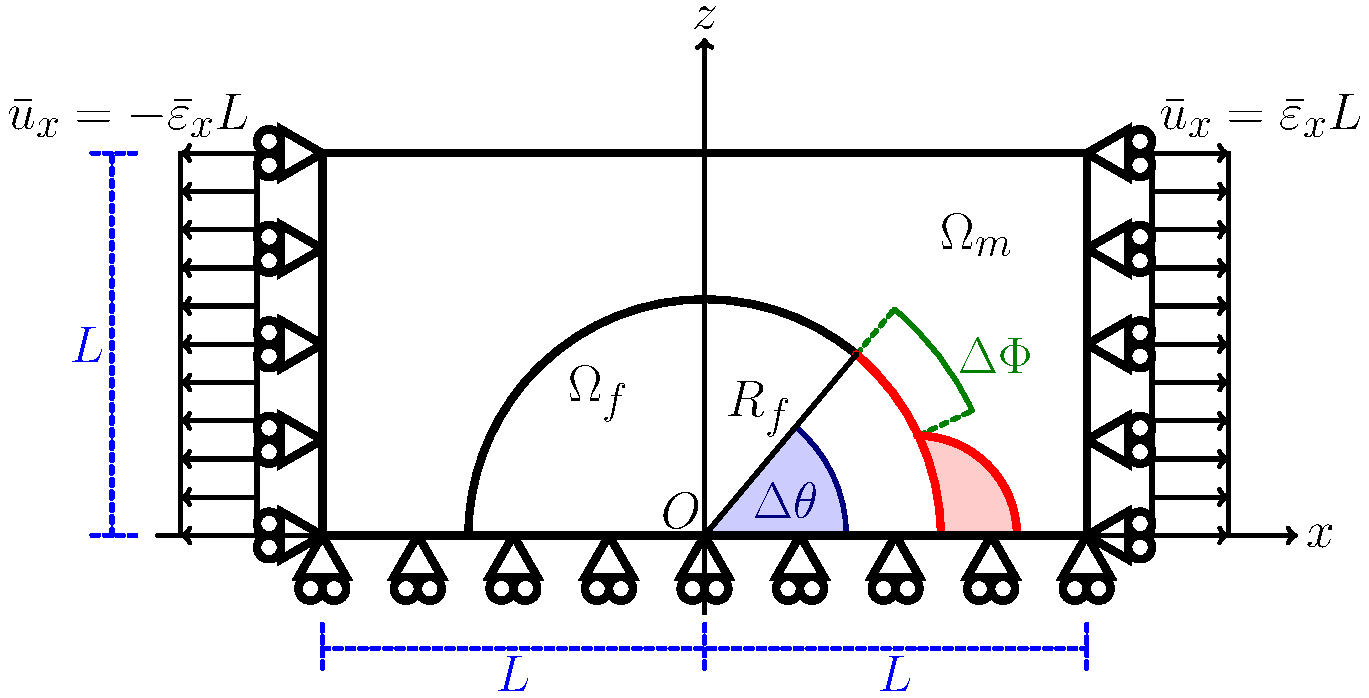
\includegraphics[width=\textwidth]{RUC.pdf}
\caption{Schematic of the model with its main parameters.}\label{fig:modelschem}
\end{figure}

As shown in Fig.~\ref{fig:modelschem}, the debond is placed symmetrically with respect to the $x$ axis and its size is characterized by the angle $\Delta\theta$ (which makes the full debond size equal to $2\Delta\theta$ and the full crack length equal to $R_{f}2{\Delta\theta}$). A region $\Delta\Phi$ of variable size appears at the crack tip for large debond sizes (at least $\geq 60^{\circ}-80^{\circ}$), in which the crack faces are in contact with each other and free to slide. Frictionless contact is thus considered between the two crack faces to allow free sliding and avoid interpenetration. Symmetry with respect to the $x$ axis is applied on the lower boundary while the upper surface is left free. Kinematic coupling on the $x$-displacement is applied along the left and right sides of the model in the form of a constant $x$-displacement $\pm\bar{\varepsilon}_{x} L$, which corresponds to transverse strain $\bar{\varepsilon}_{x}$ equal to $1\%$.

\begin{table}[!htbp]
 \centering
 \caption{Summary of the mechanical properties of fiber and matrix. $E$ stands for Young's modulus, $\mu$ for shear modulus and $\nu$ for Poisson's ratio.}
 \begin{tabular}{cccc}
\textbf{Material} & \textbf{$E\left[GPa\right]$}\ & \textbf{$\mu\left[GPa\right]$} & \textbf{$\nu\left[-\right]$} \\
\midrule
Glass fiber    & 70.0  & 29.2   & 0.2  \\
Epoxy    & 3.5    & 1.25   & 0.4
\end{tabular}
\label{tab:phaseprop}
\end{table}

The model problem is solved with the Finite Element Method (FEM) within the Abaqus environment, a commercial FEM software~\cite{abq12}. The model is meshed with second order, 2D, plane strain triangular (CPE6) and rectangular (CPE8) elements. A regular mesh of quadrilateral elements with almost unitary aspect ratio is used at the crack tip. The angular size $\delta$ of an element in the crack tip neighborhood represents the main parameter of the numerical analysis. The crack faces are modeled as element-based surfaces and a small-sliding contact pair interaction with no friction is imposed between them. The Mode I, Mode II and total Energy Release Rates (ERRs) (respectively referred to as $G_{I}$, $G_{II}$ and $G_{TOT}$) are evaluated using the VCCT~\cite{Krueger2004}, implemented in a in-house Python routine. A glass fiber-epoxy system is considered in the present work, and it is assumed that their response lies always in the linear elastic domain. The material properties of glass fiber and epoxy are reported in Table~\ref{tab:phaseprop}.

\section{Vectorial formulation of the Virtual Crack Closure Technique (VCCT)}

\subsection{Foundational relations}

In the isoparametric formulation of the Finite Element Method, the element Jacobian $J$ and its inverse $J^{-1}$ can be expressed in general as 

\begin{equation}
\underline{\underline{J}}=\begin{bmatrix}
\underline{e}_{\xi}|\underline{e}_{\eta}
\end{bmatrix}=\begin{bmatrix}
\frac{\partial x}{\partial\xi}&\frac{\partial x}{\partial\eta}\\\frac{\partial y}{\partial\xi}&\frac{\partial y}{\partial\eta}
\end{bmatrix}\qquad\underline{\underline{J}}^{-1}=\begin{bmatrix}
\underline{e}^{x}|\underline{e}^{y}
\end{bmatrix}=\begin{bmatrix}
\frac{\partial \xi}{\partial x}&\frac{\partial \xi}{\partial y}\\\frac{\partial \eta}{\partial x}&\frac{\partial \eta}{\partial y}
\end{bmatrix}
\end{equation}

where $\left\{e_{\xi}, e_{\eta}\right\}$ and $\left\{e^{x}, e^{y}\right\}$ are respectively the covariant and contravariant basis vectors of the mapping between global $\left\{x, y\right\}$ and local element $\left\{\xi, \eta\right\}$ coordinates:

\begin{equation}
\underline{e}_{\xi}=\begin{bmatrix}
\frac{\partial x}{\partial\xi}\\\frac{\partial y}{\partial\xi}
\end{bmatrix}\quad\underline{e}_{\eta}=\begin{bmatrix}
\frac{\partial x}{\partial\eta}\\\frac{\partial y}{\partial\eta}
\end{bmatrix},
\end{equation}

\begin{equation}
\underline{e}_{x}=\begin{bmatrix}
\frac{\partial \xi}{\partial x}\\\frac{\partial \eta}{\partial x}
\end{bmatrix}\quad\underline{e}_{y}=\begin{bmatrix}
\frac{\partial \xi}{\partial y}\\\frac{\partial \eta}{\partial y}
\end{bmatrix}.
\end{equation}

Denoting by $d$ the number of geometrical dimensions of the problem ($d=2$ in the present work) and by $\underline{p}$ the $d\times 1$ position vector in global coordinates, we can formally introduce the $3\left(d-1\right)\times d$ matrix operator of partial differentiation $\underline{\underline{\widetilde{B}}}$ such that

\begin{equation}\label{eq:introB}
\underline{\varepsilon}\left(\underline{p}\right)=\underline{\underline{\widetilde{B}}}\cdot\underline{u}\left(\underline{p}\right),
\end{equation}

where $\underline{u}$ and $\underline{\varepsilon}$ are respectively the $d\times 1$ displacement vector and the $3\left(d-1\right)\times 1$ strain vector in Voigt notation. Denoting by $n$ the number of nodes of a generic element ($n=s\times m$ where $s$ represents the number of sides of the element and $m$ the order of the shape functions), we can furthermore introduce the $d\times d\cdot n$ matrix \underline{\underline{N}} of shape functions such that

\begin{equation}\label{eq:introN}
\underline{u}=\underline{\underline{N}}\cdot\underline{u}_{N},
\end{equation}

where $\underline{u}_{N}$ is the $d\cdot n\times 1$ vector of element nodal variables. Having introduced $\underline{\underline{\widetilde{B}}}$ and $\underline{\underline{N}}$ in Equations~\ref{eq:introB} and~\ref{eq:introN} respectively, it is possible to define the $3\left(d-1\right)\times d\cdot n$ matrix $\underline{\underline{B}}$ of derivatives (with respect to global coordinates) of shape functions as

\begin{equation}
\underline{\underline{B}}=\underline{\underline{\widetilde{B}}}\cdot\underline{\underline{N}}.
\end{equation}

We introduce the linear elastic material behavior in the form of the $3\left(d-1\right)\times 3\left(d-1\right)$ rigidity matrix $\underline{\underline{D}}$ such that

\begin{equation}
\underline{\sigma}=\underline{\underline{D}}\cdot\underline{\varepsilon},
\end{equation}

where $\underline{\sigma}$ the $3\left(d-1\right)\times 1$ stress vector in Voigt notation. It is finally possible to define the $n\times n$ element stiffness matrix $\underline{\underline{k_{e}}}$ as 

\begin{equation}\label{eq:elestiff}
\underline{\underline{k_{e}}}=\int_{V_{e}\left(x,y\right)}\left(\underline{\underline{B}}^{T}\underline{\underline{D}}\cdot\underline{\underline{B}}\right)dV_{e}\left(x,\dots,y\right)=\int_{V_{e}\left(\xi,\eta\right)}\left(\underline{\underline{B}}^{T}\underline{\underline{D}}\cdot\underline{\underline{B}}\right)\sqrt{g}dV_{e}\left(\xi,\dots,\eta\right),
\end{equation}

where $g=det\left(\underline{\underline{J}}^{T}\underline{\underline{J}}\right)$ and $V_{e}$ is the element volume. Given that isoparametric elements are always defined between $-1$ and $1$ in each dimension, Equation~\ref{eq:elestiff} can simplified to

\begin{equation}
\underline{\underline{k_{e}}}=\int_{-1}^{1}\dots\int_{-1}^{1}\left(\underline{\underline{B}}^{T}\underline{\underline{D}}\cdot\underline{\underline{B}}\right)\sqrt{g}d\xi,\dots, d\eta,
\end{equation}

which is amenable to numerical integration by means of a Gaussian quadrature of the form

\begin{equation}\label{eq:elstiffnum}
\underline{\underline{k_{e}}}\approx \sum_{i=1}^{N}\dots\sum_{j=1}^{N}w_{i}\dots w_{j}\left(\underline{\underline{B}}^{T}\left(\xi_{i}, \dots,\eta_{j}\right)\cdot\underline{\underline{D}}\cdot\underline{\underline{B}}\left(\xi_{i}, \dots,\eta_{j}\right)\sqrt{g}\right),
\end{equation}

where $\left(\xi_{i}, \dots,\eta_{j}\right)$ are the coordinates of the $N$ Gaussian quadrature points. The element stiffness matrix as evaluated in Eq.~\ref{eq:elstiffnum} is in general a full symmetric (in the case of linear elasticity) matrix of the form

\begin{equation}
k_{e}=\begin{bmatrix}
k_{e|11}&k_{e|12}&k_{e|13}&k_{e|14}&k_{e|15}&k_{e|16}&k_{e|17}&k_{e|18}\\
k_{e|12}&k_{e|22}&k_{e|23}&k_{e|24}&k_{e|25}&k_{e|26}&k_{e|27}&k_{e|28}\\
k_{e|13}&k_{e|23}&k_{e|33}&k_{e|34}&k_{e|35}&k_{e|36}&k_{e|37}&k_{e|38}\\
k_{e|14}&k_{e|24}&k_{e|34}&k_{e|44}&k_{e|45}&k_{e|46}&k_{e|47}&k_{e|48}\\
k_{e|15}&k_{e|25}&k_{e|35}&k_{e|45}&k_{e|55}&k_{e|56}&k_{e|57}&k_{e|58}\\
k_{e|16}&k_{e|26}&k_{e|36}&k_{e|46}&k_{e|56}&k_{e|66}&k_{e|67}&k_{e|68}\\
k_{e|17}&k_{e|27}&k_{e|37}&k_{e|47}&k_{e|57}&k_{e|67}&k_{e|77}&k_{e|78}\\
k_{e|18}&k_{e|28}&k_{e|38}&k_{e|48}&k_{e|58}&k_{e|68}&k_{e|78}&k_{e|88}\\
\end{bmatrix}.
\end{equation}

\subsection{Formulation of the ERR with respect to FEM variables}

\section{Convergence analysis}

\subsection{Analytical considerations}

\subsection{Numerical results}

\section{Conclusions \& Outlook}

\section*{Acknowledgements}

Luca Di Stasio gratefully acknowledges the support of the European School of Materials (EUSMAT) through the DocMASE Doctoral Programme and the European Commission through the Erasmus Mundus Programme.

\bibliography{refs}

\end{document}
